\documentclass[border=12pt,tikz]{standalone}
\usepackage{tikz}
\usetikzlibrary{arrows.meta,shapes.geometric,calc,fit,backgrounds}

\definecolor{ink}{HTML}{1F2933}
\definecolor{ctrlcol}{HTML}{56677A}
\definecolor{idcol}{HTML}{7C3AED}
\definecolor{acccol}{HTML}{C2410C}
\definecolor{svccol}{HTML}{0F766E}
\definecolor{z1fill}{HTML}{FDECEC}
\definecolor{z1line}{HTML}{C0392B}
\definecolor{z2fill}{HTML}{F3EBFD}
\definecolor{z2line}{HTML}{7C3AED}
\definecolor{z3fill}{HTML}{E9F1FC}
\definecolor{z3line}{HTML}{1D4ED8}
\definecolor{legfill}{HTML}{F6F7F9}
\definecolor{legline}{HTML}{B7C0CC}
\definecolor{lifecol}{HTML}{9AA6B4}

\begin{document}
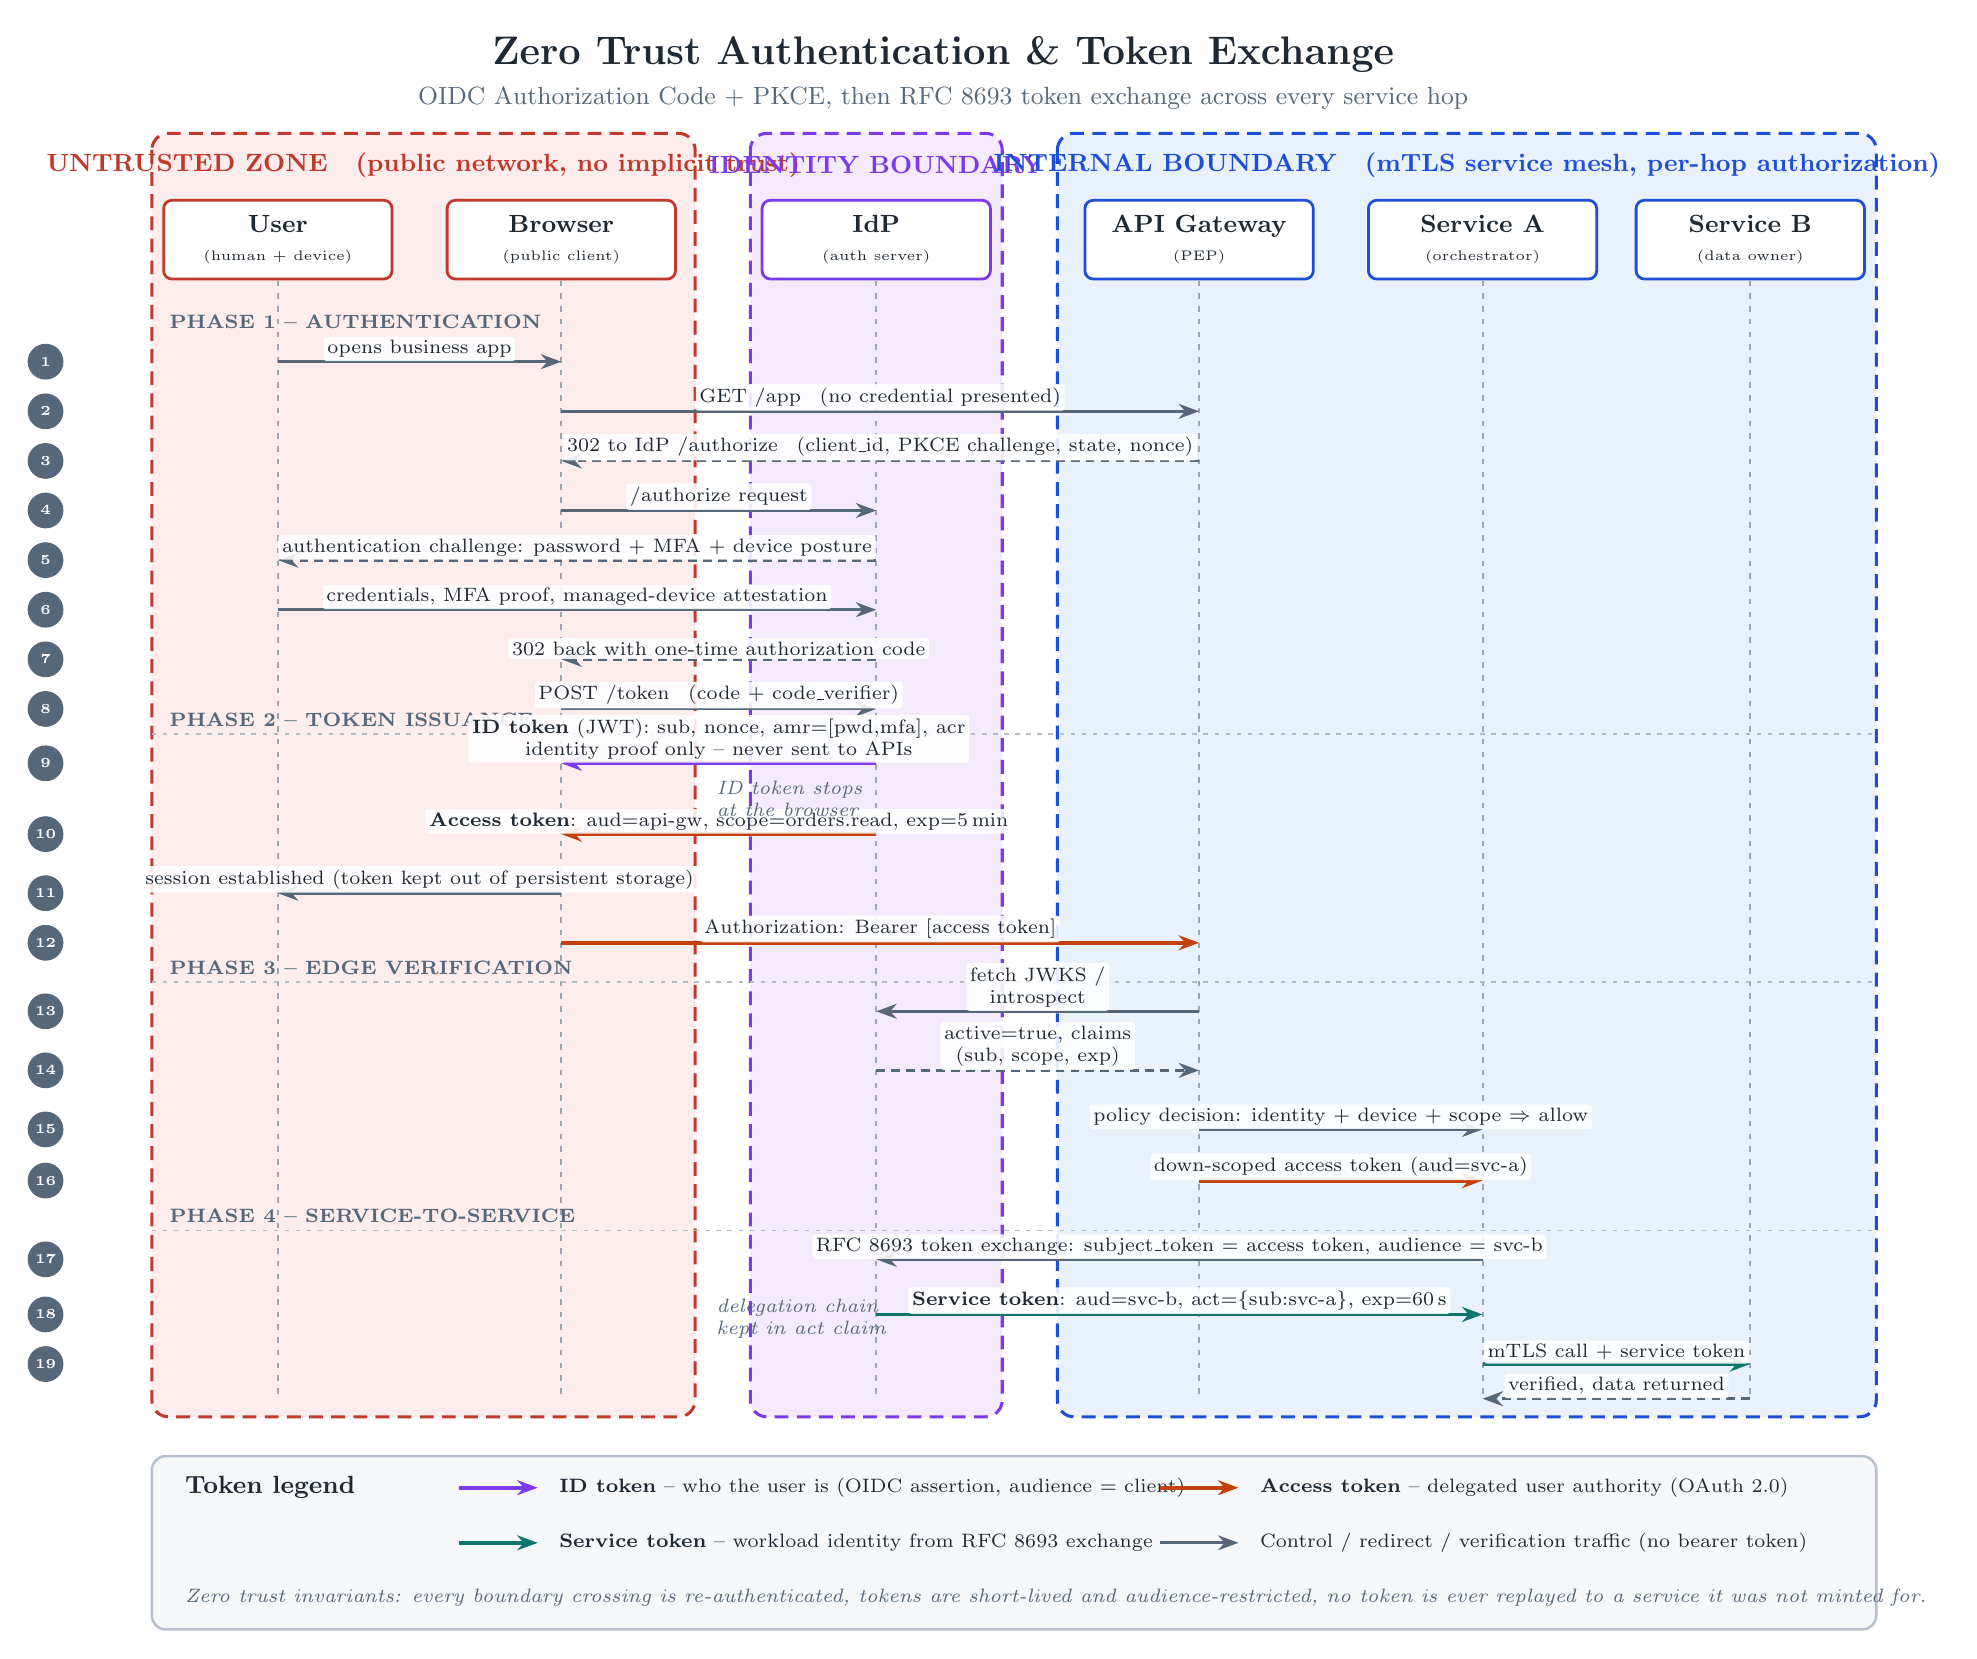
\begin{tikzpicture}[
  x=1cm,y=1cm,
  every node/.style={text=ink},
  zone/.style={rounded corners=6pt,line width=1.1pt,dash pattern=on 5pt off 3pt},
  ztitle/.style={font=\small\bfseries,align=center},
  actor/.style={draw,line width=1pt,rounded corners=3pt,fill=white,
                minimum width=2.9cm,minimum height=1.0cm,align=center,font=\small\bfseries},
  life/.style={draw=lifecol,line width=0.7pt,dash pattern=on 2pt off 2.6pt},
  msg/.style={-{Stealth[length=2.6mm,width=1.9mm]},line width=1.0pt},
  ctrl/.style={msg,draw=ctrlcol},
  ctrlb/.style={msg,draw=ctrlcol,dash pattern=on 3.2pt off 2.2pt},
  idtok/.style={msg,draw=idcol,line width=1.4pt},
  acctok/.style={msg,draw=acccol,line width=1.4pt},
  svctok/.style={msg,draw=svccol,line width=1.4pt},
  mlab/.style={font=\scriptsize,align=center,anchor=south,inner sep=1.3pt,
               fill=white,fill opacity=0.88,text opacity=1,rounded corners=1pt},
  stepb/.style={circle,draw=ctrlcol,fill=ctrlcol,text=white,inner sep=0pt,
                minimum size=4.4mm,font=\tiny\bfseries},
  note/.style={font=\scriptsize\itshape,align=left,text=ctrlcol}
]

%% ---------- helper ----------
\newcommand{\msgline}[6]{%
  \node[stepb] at (-2.95,#2) {#1};%
  \draw[#3] (#4,#2) -- (#5,#2);%
  \node[mlab] at ({(#4+#5)/2},#2) {#6};%
}

%% ---------- trust boundaries ----------
\fill[z1fill,rounded corners=6pt] (-1.60,1.35) rectangle (5.30,-14.95);
\fill[z2fill,rounded corners=6pt] (6.00,1.35) rectangle (9.20,-14.95);
\fill[z3fill,rounded corners=6pt] (9.90,1.35) rectangle (20.30,-14.95);

\draw[zone,draw=z1line] (-1.60,1.35) rectangle (5.30,-14.95);
\draw[zone,draw=z2line] (6.00,1.35) rectangle (9.20,-14.95);
\draw[zone,draw=z3line] (9.90,1.35) rectangle (20.30,-14.95);

\node[ztitle,text=z1line] at (1.85,0.95)
  {UNTRUSTED ZONE \; (public network, no implicit trust)};
\node[ztitle,text=z2line] at (7.60,0.95) {IDENTITY BOUNDARY};
\node[ztitle,text=z3line] at (15.10,0.95)
  {INTERNAL BOUNDARY \; (mTLS service mesh, per-hop authorization)};

%% ---------- title ----------
\node[font=\Large\bfseries] at (8.45,2.35) {Zero Trust Authentication \& Token Exchange};
\node[font=\small,text=ctrlcol] at (8.45,1.80)
  {OIDC Authorization Code + PKCE, then RFC 8693 token exchange across every service hop};

%% ---------- actors ----------
\node[actor,draw=z1line] (user)  at (0.00,0) {User\\[-1pt]{\tiny\mdseries (human + device)}};
\node[actor,draw=z1line] (brow)  at (3.60,0) {Browser\\[-1pt]{\tiny\mdseries (public client)}};
\node[actor,draw=z2line] (idp)   at (7.60,0) {IdP\\[-1pt]{\tiny\mdseries (auth server)}};
\node[actor,draw=z3line] (gw)    at (11.70,0) {API Gateway\\[-1pt]{\tiny\mdseries (PEP)}};
\node[actor,draw=z3line] (sva)   at (15.30,0) {Service A\\[-1pt]{\tiny\mdseries (orchestrator)}};
\node[actor,draw=z3line] (svb)   at (18.70,0) {Service B\\[-1pt]{\tiny\mdseries (data owner)}};

\foreach \x in {0.00,3.60,7.60,11.70,15.30,18.70}
  \draw[life] (\x,-0.52) -- (\x,-14.72);

%% ---------- phase separators ----------
\draw[ctrlcol!45,line width=0.5pt,dash pattern=on 1.6pt off 2.4pt]
  (-1.60,-6.28) -- (20.30,-6.28);
\draw[ctrlcol!45,line width=0.5pt,dash pattern=on 1.6pt off 2.4pt]
  (-1.60,-9.43) -- (20.30,-9.43);
\draw[ctrlcol!45,line width=0.5pt,dash pattern=on 1.6pt off 2.4pt]
  (-1.60,-12.58) -- (20.30,-12.58);

\node[font=\scriptsize\bfseries,text=ctrlcol,anchor=west,rotate=0] at (-1.50,-6.10)
  {PHASE 2 -- TOKEN ISSUANCE};
\node[font=\scriptsize\bfseries,text=ctrlcol,anchor=west] at (-1.50,-9.25)
  {PHASE 3 -- EDGE VERIFICATION};
\node[font=\scriptsize\bfseries,text=ctrlcol,anchor=west] at (-1.50,-12.40)
  {PHASE 4 -- SERVICE-TO-SERVICE};
\node[font=\scriptsize\bfseries,text=ctrlcol,anchor=west] at (-1.50,-1.05)
  {PHASE 1 -- AUTHENTICATION};

%% ---------- phase 1: authentication ----------
\msgline{1}{-1.55}{ctrl}{0.00}{3.60}{opens business app}
\msgline{2}{-2.18}{ctrl}{3.60}{11.70}{GET /app \, (no credential presented)}
\msgline{3}{-2.81}{ctrlb}{11.70}{3.60}{302 to IdP /authorize \, (client\_id, PKCE challenge, state, nonce)}
\msgline{4}{-3.44}{ctrl}{3.60}{7.60}{/authorize request}
\msgline{5}{-4.07}{ctrlb}{7.60}{0.00}{authentication challenge: password + MFA + device posture}
\msgline{6}{-4.70}{ctrl}{0.00}{7.60}{credentials, MFA proof, managed-device attestation}
\msgline{7}{-5.33}{ctrlb}{7.60}{3.60}{302 back with one-time authorization code}
\msgline{8}{-5.96}{ctrl}{3.60}{7.60}{POST /token \, (code + code\_verifier)}

%% ---------- phase 2: token issuance ----------
\msgline{9}{-6.65}{idtok}{7.60}{3.60}{\textbf{ID token} (JWT): sub, nonce, amr=[pwd,mfa], acr\\ identity proof only -- never sent to APIs}
\msgline{10}{-7.55}{acctok}{7.60}{3.60}{\textbf{Access token}: aud=api-gw, scope=orders.read, exp=5\,min}
\msgline{11}{-8.30}{ctrl}{3.60}{0.00}{session established (token kept out of persistent storage)}
\msgline{12}{-8.93}{acctok}{3.60}{11.70}{Authorization: Bearer [access token]}

%% ---------- phase 3: edge verification ----------
\msgline{13}{-9.80}{ctrl}{11.70}{7.60}{fetch JWKS /\\ introspect}
\msgline{14}{-10.55}{ctrlb}{7.60}{11.70}{active=true, claims\\ (sub, scope, exp)}
\msgline{15}{-11.30}{ctrl}{11.70}{15.30}{policy decision: identity + device + scope $\Rightarrow$ allow}
\msgline{16}{-11.95}{acctok}{11.70}{15.30}{down-scoped access token (aud=svc-a)}

%% ---------- phase 4: service-to-service ----------
\msgline{17}{-12.95}{ctrl}{15.30}{7.60}{RFC 8693 token exchange: subject\_token = access token, audience = svc-b}
\msgline{18}{-13.65}{svctok}{7.60}{15.30}{\textbf{Service token}: aud=svc-b, act=\{sub:svc-a\}, exp=60\,s}
\msgline{19}{-14.28}{svctok}{15.30}{18.70}{mTLS call + service token}

%% ---------- return path ----------
\draw[ctrlb] (18.70,-14.72) -- (15.30,-14.72);
\node[mlab] at (17.00,-14.72) {verified, data returned};

%% ---------- annotations ----------
\node[note,anchor=west] at (5.45,-7.10) {ID token stops\\at the browser};
\node[note,anchor=west] at (5.45,-13.70) {delegation chain\\kept in act claim};

%% ---------- legend ----------
\fill[legfill,rounded corners=5pt] (-1.60,-15.45) rectangle (20.30,-17.65);
\draw[legline,line width=0.9pt,rounded corners=5pt] (-1.60,-15.45) rectangle (20.30,-17.65);

\node[font=\small\bfseries,anchor=west] at (-1.30,-15.85) {Token legend};

\draw[idtok] (2.30,-15.85) -- (3.30,-15.85);
\node[font=\scriptsize,anchor=west] at (3.45,-15.85)
  {\textbf{ID token} -- who the user is (OIDC assertion, audience = client)};

\draw[acctok] (11.20,-15.85) -- (12.20,-15.85);
\node[font=\scriptsize,anchor=west] at (12.35,-15.85)
  {\textbf{Access token} -- delegated user authority (OAuth 2.0)};

\draw[svctok] (2.30,-16.55) -- (3.30,-16.55);
\node[font=\scriptsize,anchor=west] at (3.45,-16.55)
  {\textbf{Service token} -- workload identity from RFC 8693 exchange};

\draw[ctrl] (11.20,-16.55) -- (12.20,-16.55);
\node[font=\scriptsize,anchor=west] at (12.35,-16.55)
  {Control / redirect / verification traffic (no bearer token)};

\node[font=\scriptsize\itshape,text=ctrlcol,anchor=west] at (-1.30,-17.25)
  {Zero trust invariants: every boundary crossing is re-authenticated, tokens are short-lived and
   audience-restricted, no token is ever replayed to a service it was not minted for.};

\end{tikzpicture}
\end{document}
